
\section{HSI (Horizontal Situation Indicator) Indicador de situación horizontal}

Uno de los instrumentos que pueden realizar la función de indicadores VOR, es el HSI.

El HSI o indicador de situación horizontal, es uno de los componentes del Director de Vuelo (FLIGHT DIRECTOR) y actúa como instrumento indicador para las señales de radionavegación que llegan a bordo de la aeronave. Este instrumento puede también ser instalado independientemente del sistema Director de Vuelo y es susceptible de ser usado como indicador de las estaciones VOR, ILS y ADF.

Por otra parte, el HSI presenta las indicaciones de sistemas como el CLC 3D, el INS, el OMEGA y el DOPPLER, sirviendo las órdenes de las computadoras de navegación de estos equipos.


\begin{figure}[!h]
  \centering
  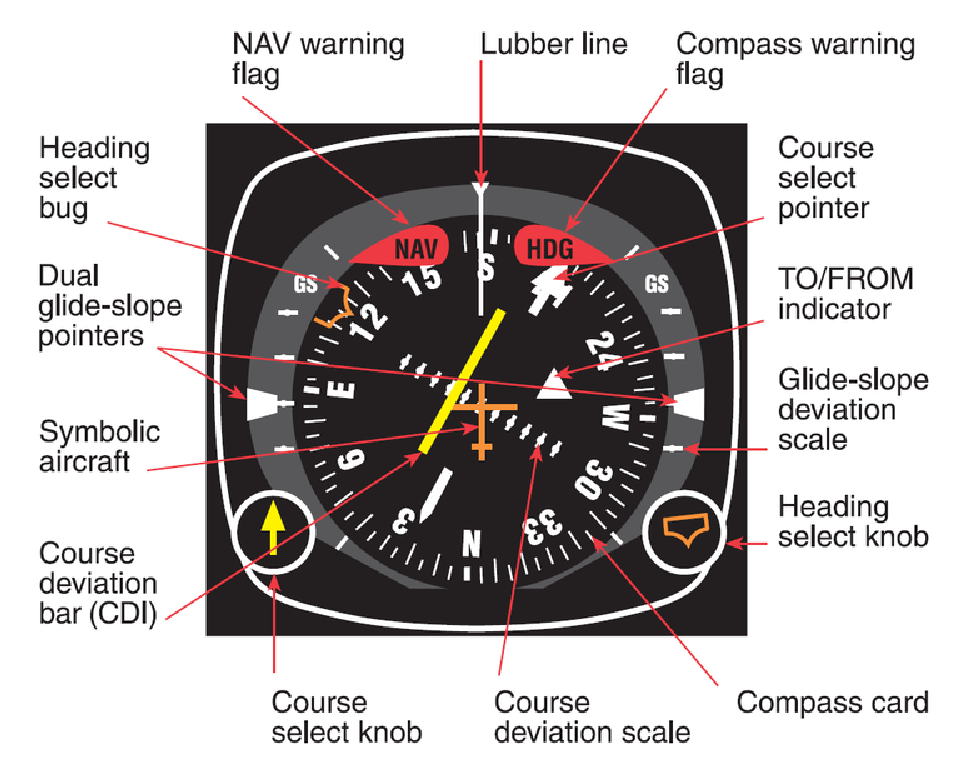
\includegraphics[keepaspectratio,width=0.7\textwidth]{Imagenes/06.02.vor.imagenes/Wiki-HSI.eps}
  \caption{Partes de un HSI (gentileza Federal Aviation Administration )}
  \label{fig:HSI-partes}
\end{figure}

Los elementos que componen el HSI son:

\subsection{Rosa de rumbos (compass card) }

Actúa de la misma forma que el girodireccional del avión y está sincronizada con el sistema de brújula giroestabilizada del mismo. Bajo el índice superior del instrumento, se leerá siempre el rumbo magnético que lleve la aeronave. Las divisiones de la rosa son las mismas que las descritas para los indicadores de ADF.

\subsection{CDI  (Course Deviation Indicator, Indicador Desviación de Curso)}

La situación del avión con respecto a cualquier ruta seleccionada, se muestra gráficamente, pues, el CDI es totalmente móvil, pudiendo adoptar cualquier posición.

A ambos extremos del CDI están los indicadores de ruta selectada y de ruta recíproca. El primero de ellos tiene 1a forma de una pequeña espada e indica siempre la ruta seleccionada. El segundo indicador es el de ruta recíproca.

El selector de rutas OBS, es el mando situado en la parte inferior izquierda, en la Figura anterior, de la caja dell instrumento. Mediante una serie de transmisiones mecánicas hace girar a los indicadores de ruta selectada y recíproca. Naturalmente, a l ser girado el OBS. eI CDI también variara su posición en el interior del instrumento.

\subsection{Indicador TO-FROM}

Un sencillo triángulo situado en el centro del instrumento indica si se está volando en TO o en FROM.

Cuando el triángulo está al mismo lado que la espada indicadora de ruta selectada el avión vuela en TO. Por el contrario, si el triángulo apareciera al lado en el que está el indicador de ruta recíproca, se estaría volando en FROM.

\subsection{Puntos de referencia}

\begin{enumerate}

\item Existen ocho puntos de referencia situados cada 45 grados alrededor de la rosa de rumbos.

\item Un triángulo invertido en la parte superior de la caja del instrumento y un pequeño segmento en la parte inferior, constituyen las referencias de rumbo magnético y su recíproco, que lleva el avión.

\item Cinco puntos en el centro del instrumento indican el desplazamiento en grados del CDI. El valor en grados de cada punto es el mismo que en el instrumento VOR convencional. Cuando el HSI actúa como indicador de ILS, el valor de cada punto se reduce de la misma manera que en el indicador ILS clásico. 

\item También en el centro del instrumento va dibujado un pequeño avión que indica la posición relativa de éste con respecto a la ruta selectada.

\item Con eI mando instalado en la parte inferior derecha del HSI (Figura \ref{fig:HSI-partes}, Heading select knob), se hace girar la referencia situada sobre la rosa de rumbos. EI dibujo que lleva rotulado este mando tiene la misma forma que Ia referencia móvil. Esta es usada por el piloto como recordatorio de cualquier ruta o rumbo, aunque en realidad es un selector de rumbos para que el piloto automático (AUTO PILOT) inicie su seguimiento.

\end{enumerate}

\subsection{Indicaci\'on de senda de planeo}

En ambos lados del HSI va colocado el GSI (Glide Slope Indicator, Indicador de Senda de Planeo), mediante punteros que señalan la senda de planeo (dual glide-slope pointers).

El GSI entra en funcionamiento cuando el instrumento actúa como indicador de ILS (Instrument Landing System, Sistema de Aterrizaje por Instrumentos).

Un par de pequeños triángulos se desplazarán por encima o por debajo de un fiel indicando la posición del avión con relación a la senda de planeo de una instalación ILS. Los puntos blancos indican el desplazamiento en grados del GSI. 

Otros tipos de HSI tienen una distribución distinta de los elementos descriptos, pero básicamente son los mismos.


\begin{figure}[!h]
  \centering
  \subfigure[EHSI-4000 (Gentileza      L-3 Avionics Systems   )]{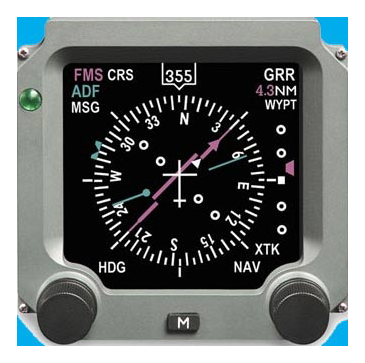
\includegraphics[keepaspectratio,width=0.45\textwidth]{Imagenes/06.02.vor.imagenes/hsi_ehsi-4000.eps}}
\subfigure[HSI Bendix/King KI-825 (Gentileza Bendix)]{
\includegraphics[keepaspectratio,width=0.45\textwidth]{Imagenes/06.02.vor.imagenes/hsi-Bendix-King-KI-825.eps}}
  \caption{Tipos de HSI}
\end{figure}



En las Figuras anteriores pueden apreciarse HSI con pantalla de tipo Active Matrix Liquid Crystal Display (AMLCD), que resulta visible tanto con luz solar directa como en una cabina a oscuras.

\begin{enumerate}

\item En una de las esquinas va instalado el indicador del equipo radiotelemétrico (DME) dando información constante de la distancia que separa al avión de la estación selectada.


\item En una ventanilla aparece la ruta selectada mediante el OBS. 


\item Por último, en este HSI pueden verse dos referencias más, en distinto color que no son más que la cabeza y la cola de una aguja indicadora de ADF. Al ser Ia carta de HSI móvil, esta aguja trabajará como si el instrumento fuera un RMI.

\end{enumerate}



